% ============================================================
%  WanderMate -- Project 3 Task 3 Deliverable
%  Team 8 · S26CS6.401 Software Engineering
%  Architectural Tactics & Design Patterns
% ============================================================
\documentclass[12pt, a4paper]{article}

% ── Packages ────────────────────────────────────────────────
\usepackage[a4paper, top=2.5cm, bottom=2.5cm,
            left=2.8cm, right=2.8cm, headheight=15pt]{geometry}
\usepackage[utf8]{inputenc}
\usepackage[T1]{fontenc}
\usepackage{xcolor}
\usepackage{titlesec}
\usepackage{titletoc}
\usepackage{fancyhdr}
\usepackage{graphicx}
\usepackage{booktabs}
\usepackage{longtable}
\usepackage{array}
\usepackage{tabularx}
\usepackage{multirow}
\usepackage{colortbl}
\usepackage{enumitem}
\usepackage{mdframed}
\usepackage{tcolorbox}
\usepackage{hyperref}
\usepackage{parskip}
\usepackage{setspace}
\usepackage{ragged2e}
\usepackage{amsmath}
\usepackage{float}

\tcbuselibrary{skins, breakable}

% ── Colour Palette (matching task1 formal style) ────────────
\definecolor{headingblack}{HTML}{1A1A1A}
\definecolor{rulegray}{HTML}{888888}
\definecolor{tableheaderbg}{HTML}{2C2C2C}
\definecolor{tablealtbg}{HTML}{F5F5F5}
\definecolor{notebg}{HTML}{F7F7F7}
\definecolor{noteborder}{HTML}{AAAAAA}
\definecolor{bodytext}{HTML}{1A1A1A}
\definecolor{captiontext}{HTML}{444444}
\definecolor{linkcolor}{HTML}{000000}

% ── Hyperref ────────────────────────────────────────────────
\hypersetup{
    colorlinks=false,
    hidelinks,
    pdftitle={Project 3 Task 3 -- Architectural Tactics and Design Patterns},
    bookmarksnumbered=true,
}

% ── Section Formatting ──────────────────────────────────────
\titleformat{\section}
  {\large\bfseries\color{headingblack}}
  {\thesection.}{0.6em}{}
  [\vspace{0.1em}\textcolor{rulegray}{\titlerule[0.4pt]}\vspace{0.2em}]

\titleformat{\subsection}
  {\normalsize\bfseries\color{headingblack}}
  {\thesubsection}{0.6em}{}

\titleformat{\subsubsection}
  {\normalsize\bfseries\itshape\color{headingblack}}
  {\thesubsubsection}{0.6em}{}

\titlespacing{\section}{0pt}{16pt}{6pt}
\titlespacing{\subsection}{0pt}{12pt}{4pt}
\titlespacing{\subsubsection}{0pt}{8pt}{3pt}

% ── Table Column Types ──────────────────────────────────────
\newcolumntype{L}[1]{>{\RaggedRight\arraybackslash}p{#1}}
\newcolumntype{C}[1]{>{\centering\arraybackslash}p{#1}}

% ── Note / Callout Box ──────────────────────────────────────
\tcbset{
  notebox/.style={
    enhanced,
    breakable,
    colback=notebg,
    colframe=noteborder,
    leftrule=2pt,
    toprule=0.3pt,
    bottomrule=0.3pt,
    rightrule=0.3pt,
    arc=0pt,
    boxsep=2pt,
    left=8pt, right=6pt, top=5pt, bottom=5pt,
    fontupper=\small\color{bodytext},
  }
}

% ── Paragraph / List spacing ────────────────────────────────
\setlist[itemize]{leftmargin=1.6em, itemsep=1pt,
                  parsep=0pt, topsep=3pt, label=\textendash}
\setlist[enumerate]{leftmargin=1.6em, itemsep=1pt, parsep=0pt, topsep=3pt}
\setlength{\parskip}{4pt}
\setlength{\parindent}{0pt}

% ── Convenience macros ──────────────────────────────────────
\newcommand{\thcell}[1]{\textcolor{white}{\textbf{\small #1}}}
\renewcommand{\arraystretch}{1.3}
\newcommand{\code}[1]{\texttt{\small #1}}

% ============================================================
\begin{document}

% ── Title Page ──────────────────────────────────────────────
\thispagestyle{empty}

\begin{center}
  {\LARGE\bfseries WanderMate: Social Mobile Travel Planner}\\[0.8em]
  {\large Task 3}\\[0.4em]
  {\large Architectural Tactics \& Design Patterns}
\end{center}

% ── Table of Contents ───────────────────────────────────────
\tableofcontents
\newpage

% ============================================================
\section{Introduction}
% ============================================================

WanderMate is a social, collaborative mobile travel planner built as a React Native (Expo) frontend communicating with a Node.js/Express backend, backed by MongoDB for persistent storage and Firebase Realtime Database for real-time event propagation. The system integrates multiple external APIs --- Google Places (POI discovery), OpenRouteService (routing and optimization), and Overpass/OSM (disabled fallback) --- all proxied through a backend API Gateway.

The architecture must simultaneously satisfy demanding non-functional requirements spanning \textbf{performance}, \textbf{security}, \textbf{availability}, \textbf{scalability}, and \textbf{modifiability}, while operating within the economic constraints of free-tier API quotas. This document catalogues the \textbf{five architectural tactics} and \textbf{two design patterns} that form the backbone of WanderMate's architectural strategy, linking each to specific NFRs and illustrating their implementation with diagrams.

\begin{tcolorbox}[notebox]
  \textbf{Notation.} Throughout this document, requirement identifiers such as \textsc{NFR-06} and \textsc{FR-07} refer to the requirements defined in the Task~1 deliverable. Code references use \code{monospace} font and point to files in the WanderMate repository.
\end{tcolorbox}

% ============================================================
\section{Architectural Tactics}
% ============================================================

Architectural tactics are fundamental design decisions that directly influence a system's quality attributes. Each tactic below addresses one or more non-functional requirements and is implemented in specific components of the WanderMate codebase.

% -----------------------------------------------------------
\subsection{Tactic 1: Multi-layer Response Caching}
% -----------------------------------------------------------

\subsubsection{Description}

Response caching is a \textbf{performance tactic} that reduces latency and resource consumption by storing the results of expensive computations or external API calls and serving them directly on subsequent identical requests, bypassing the original computation entirely. WanderMate implements caching at \emph{three distinct architectural layers}, creating a defence-in-depth strategy against latency spikes and API quota exhaustion.

\subsubsection{Non-Functional Requirements Addressed}

\begin{itemize}
  \item \textbf{NFR-01 (Performance)} --- Ensures POI search results and map data are returned within the 2-second target at p95 by serving cached responses for repeated queries.
  \item \textbf{NFR-06 (Scalability / Quota Compliance)} --- Minimises outbound calls to Google Places ($\leq$ 5{,}000 req/month) and ORS ($\leq$ 2{,}000 req/day) by caching responses with calibrated TTLs, ensuring zero overage cost at launch.
  \item \textbf{NFR-07 (Availability)} --- Client-side caching via AsyncStorage allows itinerary data to be read even when the device is completely offline.
\end{itemize}

\subsubsection{Implementation Details}

\begin{longtable}{C{1.8cm} L{3.8cm} L{4.0cm} L{3.5cm}}
\toprule
\rowcolor{tableheaderbg}
\thcell{Layer} & \thcell{Technology} & \thcell{Scope \& TTL} & \thcell{Code Location} \\
\midrule
\endhead
\bottomrule
\endfoot

\textbf{L1: Client} & AsyncStorage via \code{localCache} module & Trip data (infinite TTL offline), general cache (1~hour default TTL) & \code{frontend/services/syncQueue.ts} \\

\rowcolor{tablealtbg}
\textbf{L2: Service} & In-process \code{node-cache} inside TravelService & POI search: 30~min, Place details: 24~hr, Routes: 1~hr & \code{backend/src/services/travelService.js} \\

\textbf{L3: Middle\-ware} & Express middleware \code{cacheMiddleware} & Per-route response cache with configurable TTL (default 1~hr) & \code{backend/src/middleware/cache.js} \\

\end{longtable}

\subsubsection{Caching Flow Diagram}

\begin{figure}[H]
\centering
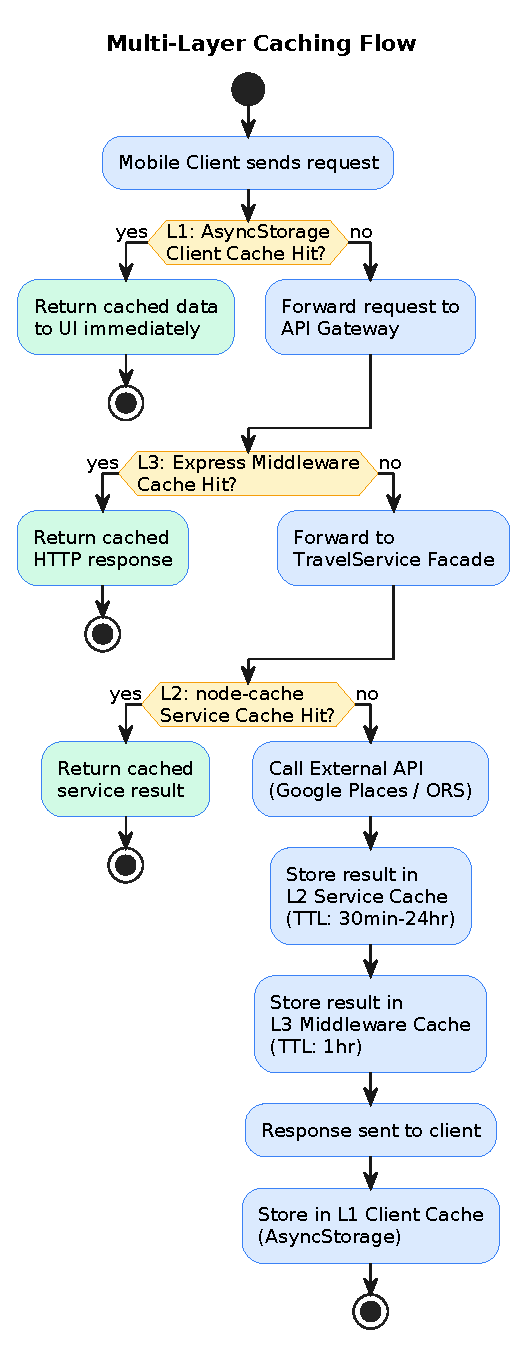
\includegraphics[width=0.65\textwidth]{caching_flow.pdf}
\caption{Multi-layer caching flow: requests traverse L1 (client), L2 (service), and L3 (middleware) caches before reaching external APIs.}
\label{fig:caching-flow}
\end{figure}

\subsubsection{Reasoning}

The three-layer caching strategy is calibrated to the specific cost and latency characteristics of each external API. Google Places, with its restrictive free-tier quota (5{,}000 requests/month), receives the longest cache TTL for place details (24~hours), because details data (address, opening hours, photos) changes infrequently. Route calculations via ORS receive a moderate TTL (1~hour), balancing freshness against the daily quota cap. Client-side caching with infinite TTL during offline mode satisfies NFR-07 by ensuring previously viewed trips remain accessible without network connectivity.

% -----------------------------------------------------------
\subsection{Tactic 2: Authentication \& Secret Proxying}
% -----------------------------------------------------------

\subsubsection{Description}

Authentication and secret proxying is a \textbf{security tactic} that prevents unauthorised access and protects sensitive credentials from exposure. WanderMate employs a dual-layer security model: \emph{Firebase JWT token verification} authenticates every API request, and the \emph{API Gateway pattern} ensures that all third-party API keys reside exclusively on the server, never reaching the mobile client bundle.

\subsubsection{Non-Functional Requirements Addressed}

\begin{itemize}
  \item \textbf{NFR-10 (Security / Transport)} --- All client--server communication uses HTTPS with TLS 1.2+. The API Gateway additionally applies Helmet security headers to every response.
  \item \textbf{NFR-11 (Security / Secret Protection)} --- Third-party API keys (Google Places, ORS) are stored as server-side environment variables in \code{.env} and are never transmitted to the client. All calls to external services are proxied through the backend gateway.
  \item \textbf{NFR-12 (Security / Authorisation)} --- Per-trip access control (ownership + collaborator checks) is enforced at the API layer, preventing horizontal privilege escalation.
\end{itemize}

\subsubsection{Implementation Details}

\begin{enumerate}
  \item \textbf{Token-based Authentication}: The \code{authenticate} middleware (\code{backend/src/middleware/auth.js}) extracts the Bearer token from the \code{Authorization} header of every request and verifies it using Firebase Admin SDK's \code{verifyIdToken()} method. The decoded claims (UID, email, display name) are attached to \code{req.user} for downstream route handlers.

  \item \textbf{Client-side Token Injection}: The Axios request interceptor in \code{frontend/services/api.ts} automatically attaches the current user's Firebase ID token to every outbound API call, ensuring seamless authentication without manual token management in UI components.

  \item \textbf{Secret Vault}: All third-party API keys (\code{GOOGLE\_PLACES\_API\_KEY}, \code{ORS\_API\_KEY}) are loaded from environment variables in the backend process. The mobile client communicates only with the WanderMate API Gateway; it has no knowledge of --- and no access to --- external API credentials.

  \item \textbf{HTTP Security Headers}: The \code{helmet} middleware is applied globally to set \code{X-Content-Type-Options}, \code{X-Frame-Options}, \code{Strict-Transport-Security}, and other protective headers on every response.
\end{enumerate}

\subsubsection{Security Architecture Diagram}

\begin{figure}[H]
\centering
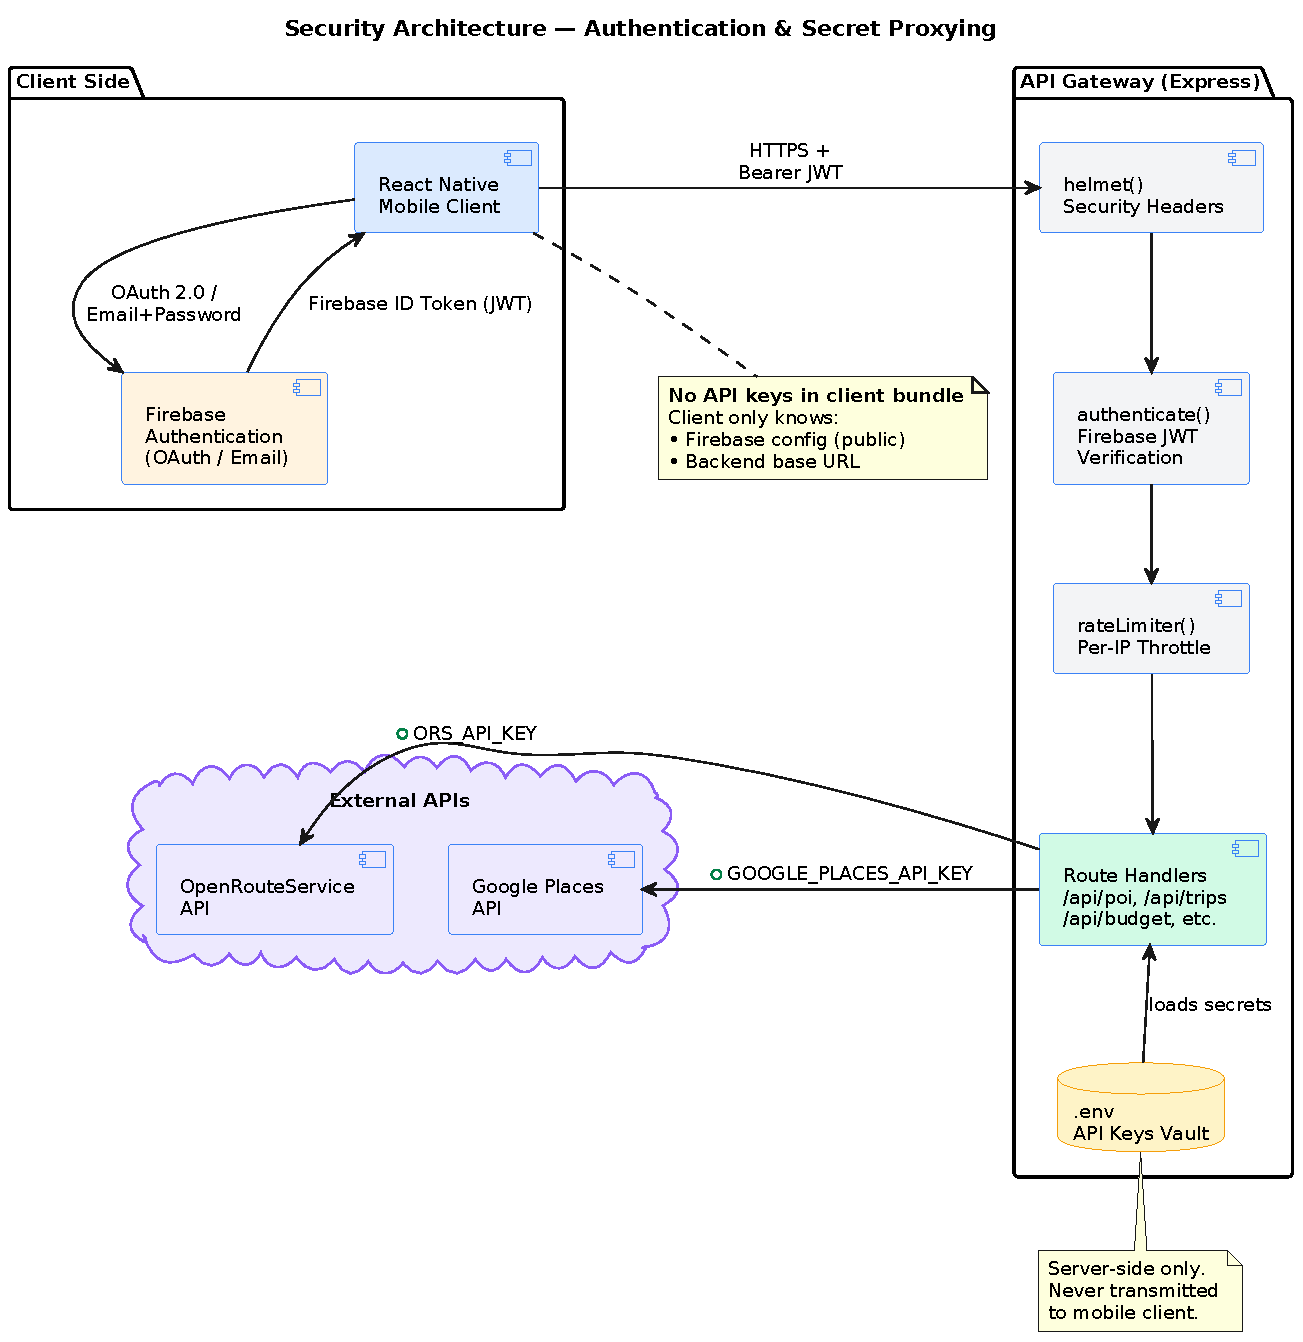
\includegraphics[width=0.85\textwidth]{security_architecture.pdf}
\caption{Security architecture: the mobile client authenticates via Firebase JWT tokens; all external API calls are proxied through the backend gateway which injects API keys from server-side environment variables. Direct client-to-external-API communication is blocked by design.}
\label{fig:security-arch}
\end{figure}

\subsubsection{Reasoning}

Embedding API keys in a mobile application bundle is a well-documented anti-pattern: reverse engineering tools (e.g., \code{apktool}) can extract keys from Android APKs in minutes. By routing all external API calls through the backend gateway, WanderMate ensures that keys are stored only in server memory. The gateway simultaneously serves as a centralised enforcement point for authentication, rate limiting, and caching --- three concerns that would be fragmented and unreliable if handled on the client side.

% -----------------------------------------------------------
\subsection{Tactic 3: Rate Limiting \& Throttling}
% -----------------------------------------------------------

\subsubsection{Description}

Rate limiting is a \textbf{scalability tactic} that controls the volume of requests processed per unit of time, protecting both the system's own resources and the quotas of external services. WanderMate applies rate limiting at two granularities: a \emph{general limiter} for all API endpoints and a stricter \emph{external API limiter} for routes that proxy requests to third-party services.

\subsubsection{Non-Functional Requirements Addressed}

\begin{itemize}
  \item \textbf{NFR-04 (Scalability)} --- Prevents any single user from monopolising server resources, ensuring the gateway can sustain 200 concurrent users.
  \item \textbf{NFR-06 (Quota Compliance)} --- The external API rate limiter directly caps the number of outbound calls to Google Places and ORS, guaranteeing zero overage cost at launch.
\end{itemize}

\subsubsection{Implementation Details}

\begin{longtable}{L{3.0cm} C{2.5cm} C{2.5cm} L{5.0cm}}
\toprule
\rowcolor{tableheaderbg}
\thcell{Limiter} & \thcell{Window} & \thcell{Max Requests} & \thcell{Scope / Applied To} \\
\midrule
\endhead
\bottomrule
\endfoot

\code{generalLimiter} & 15 minutes & 100 per IP & All \code{/api/*} endpoints (global middleware in \code{index.js}) \\

\rowcolor{tablealtbg}
\code{externalApiLimiter} & 1 hour & 50 per IP & POI search, category browsing, place details, route calculation (applied per-route in \code{poi.js} and \code{routes.js}) \\

\end{longtable}

Both limiters use the \code{express-rate-limit} library with \code{standardHeaders: true} (returning \code{RateLimit-*} response headers) and \code{legacyHeaders: false}. When a client exceeds the limit, the middleware returns a JSON error response:

\begin{verbatim}
  HTTP 429 Too Many Requests
  { "error": "Too many requests, please try again later" }
\end{verbatim}

\subsubsection{Reasoning}

The dual-tier rate limiting strategy reflects the asymmetric cost structure of WanderMate's backend operations. Internal operations (trip CRUD, budget management) are cheap --- they hit only MongoDB. External operations (POI search, route optimisation) incur real costs against finite free-tier quotas. By applying a much tighter limit (50 req/hour) to external API proxying routes, the system ensures that even under aggressive usage patterns, daily/monthly quotas are not exhausted. The general limiter (100 req/15 min) serves as a broad denial-of-service mitigation layer, protecting the Express event loop from resource exhaustion.

% -----------------------------------------------------------
\subsection{Tactic 4: Graceful Degradation \& Fallback}
% -----------------------------------------------------------

\subsubsection{Description}

Graceful degradation is an \textbf{availability tactic} that ensures the system continues to provide useful functionality when individual components or external dependencies fail. Rather than surfacing errors or blank screens to users, the system falls back to alternative data sources or cached data, providing a degraded but functional experience.

\subsubsection{Non-Functional Requirements Addressed}

\begin{itemize}
  \item \textbf{NFR-07 (Availability / Offline-first)} --- Core itinerary viewing and editing remain available when the device is offline, using AsyncStorage-backed local cache and a sync queue for pending mutations.
  \item \textbf{NFR-08 (Reliability / API Failure)} --- When Google Places API is unavailable, POI search degrades gracefully to ORS POI results with zero user-facing crashes.
  \item \textbf{NFR-09 (Reliability / Error Handling)} --- Every failure scenario returns a structured JSON error response; uncaught exceptions are captured by the global Express error handler.
\end{itemize}

\subsubsection{Implementation Details}

WanderMate implements graceful degradation at three levels:

\begin{enumerate}
  \item \textbf{Server-side Provider Fallback}: The \code{TravelService.searchPOI()} method wraps the Google Places API call in a \code{try/catch}. On failure (network timeout, quota exhaustion, invalid response), it silently falls through to the ORS POI endpoint:

  \begin{verbatim}
    results = await this.places.searchPOI(...)
                     .catch(err => { return []; });
    if (results.length === 0) {
        results = await this.ors.searchPOI(...)
                       .catch(err => { return []; });
    }
  \end{verbatim}

  \item \textbf{Client-side Offline Fallback}: Every Zustand store method (e.g., \code{fetchTrips}, \code{fetchTrip}) first attempts an API call. On failure, it reads from \code{localCache} (AsyncStorage) with infinite TTL, displaying the last-known state:

  \begin{verbatim}
    try { response = await api.get('/trips'); }
    catch {
        const cached = await localCache.get('trips', Infinity);
        if (cached) set({ trips: cached });
    }
  \end{verbatim}

  \item \textbf{Mutation Queuing}: When write operations fail (offline or server error), the \code{syncQueue} persists the pending mutation to AsyncStorage. On reconnect, the queue flushes in timestamp order, ensuring eventual consistency:

  \begin{verbatim}
    catch (error) {
        await syncQueue.add({
          method: 'POST',
          url: '/trips',
          data
        });
    }
  \end{verbatim}
\end{enumerate}

\subsubsection{Degradation Flow Diagram}

\begin{figure}[H]
\centering
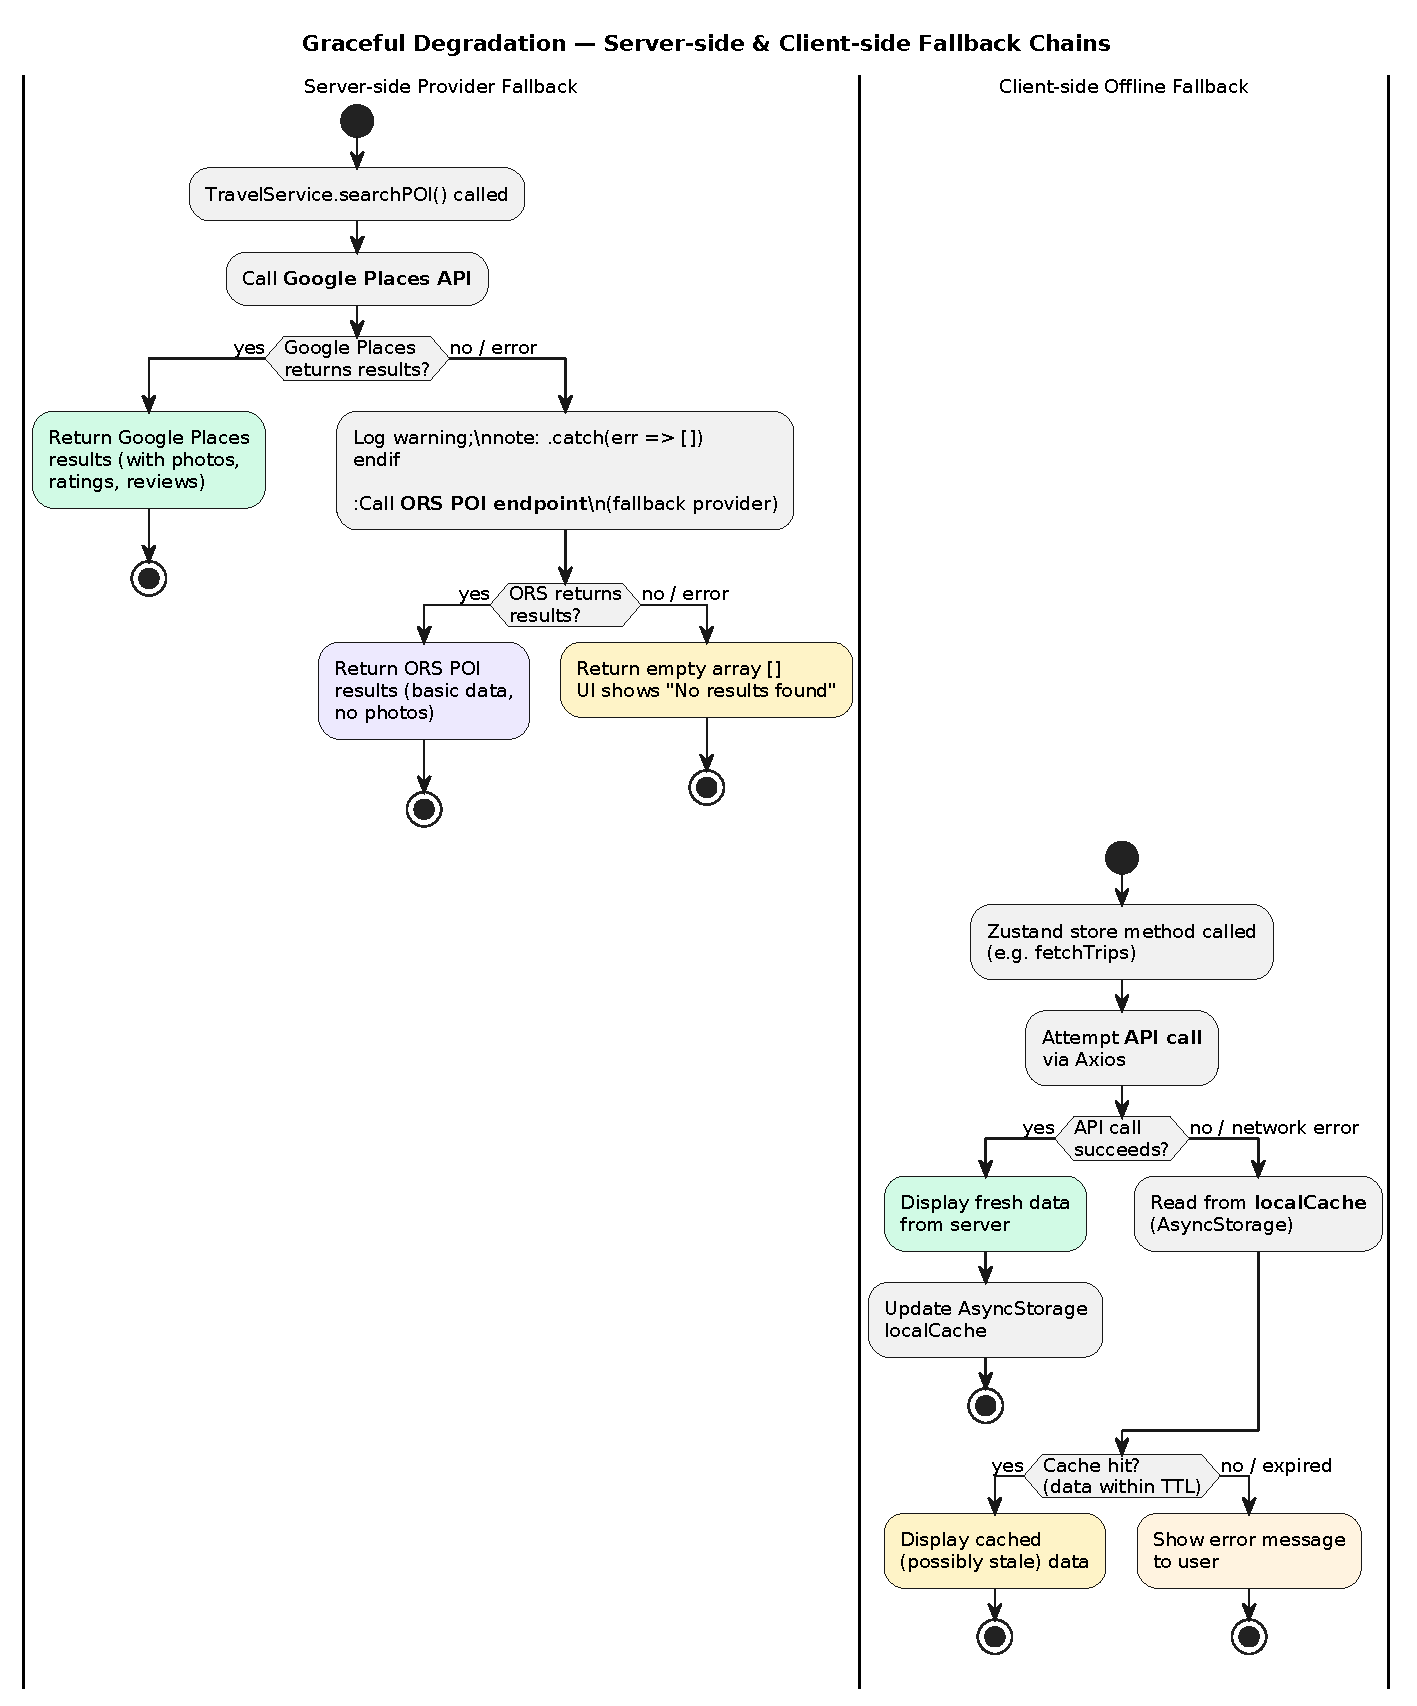
\includegraphics[width=0.65\textwidth]{degradation_flow.pdf}
\caption{Graceful degradation chains. Left: server-side POI provider fallback (Google Places $\to$ ORS $\to$ empty). Right: client-side offline fallback (API $\to$ AsyncStorage cache $\to$ error message).}
\label{fig:degradation}
\end{figure}

\subsubsection{Reasoning}

Travel applications must remain usable in environments with intermittent connectivity (airports, remote destinations, underground transport). By treating offline access as a \emph{first-class architectural concern} rather than an edge case, WanderMate ensures that users can always view and edit their itineraries. The server-side provider fallback chain prevents a single external API outage from rendering the entire POI discovery feature unusable --- a critical resilience property for a system that depends on third-party services.

% -----------------------------------------------------------
\subsection{Tactic 5: Separation of Concerns via Layered Architecture}
% -----------------------------------------------------------

\subsubsection{Description}

Separation of concerns is a \textbf{modifiability tactic} that partitions the system into layers with well-defined responsibilities and strict dependency direction. Each layer communicates only with its immediate neighbours, preventing cross-layer coupling and enabling independent evolution of UI, business logic, and data access code.

\subsubsection{Non-Functional Requirements Addressed}

\begin{itemize}
  \item \textbf{NFR-14 (Maintainability / Modularity)} --- The codebase is organised into independently testable modules aligned with subsystem boundaries, with module fan-out constrained to fewer than 5 dependencies per module.
  \item \textbf{NFR-15 (Maintainability / Provider Swappability)} --- Swapping the POI provider requires changes only within the TravelService Facade and the specific adapter module; no changes to UI screens, routes, or stores are necessary.
\end{itemize}

\subsubsection{Implementation Details}

WanderMate employs a four-layer architecture on both the backend and frontend:

\vspace{0.4em}
\textbf{Backend layers (Node.js / Express):}
\begin{enumerate}
  \item \textbf{Presentation Layer} --- Express Route Handlers (\code{trips.js}, \code{poi.js}, \code{budget.js}, \code{feed.js}, \code{users.js}, \code{routes.js})
  \item \textbf{Business Logic Layer} --- TravelService Facade, TripObserver (EventEmitter)
  \item \textbf{Data Access Layer} --- Mongoose Models (\code{Trip}, \code{Expense}, \code{FeedPost}, \code{User})
  \item \textbf{Infrastructure Layer} --- Config, Middleware (\code{auth}, \code{cache}, \code{rateLimiter}), Firebase Admin SDK
\end{enumerate}

\textbf{Frontend layers (React Native / Expo):}
\begin{enumerate}
  \item \textbf{View Layer} --- React Native Screens and Components (\code{app/}, \code{components/})
  \item \textbf{State Management Layer} --- Zustand Stores (\code{tripStore}, \code{budgetStore}, \code{feedStore}, \code{authStore})
  \item \textbf{Service Layer} --- API Client (\code{api.ts}), Sync Queue (\code{syncQueue.ts}), Local Cache
  \item \textbf{Infrastructure Layer} --- Firebase SDK (\code{config/firebase.ts}), AsyncStorage, Env Config
\end{enumerate}

\subsubsection{Layered Architecture Diagram}

\begin{figure}[H]
\centering
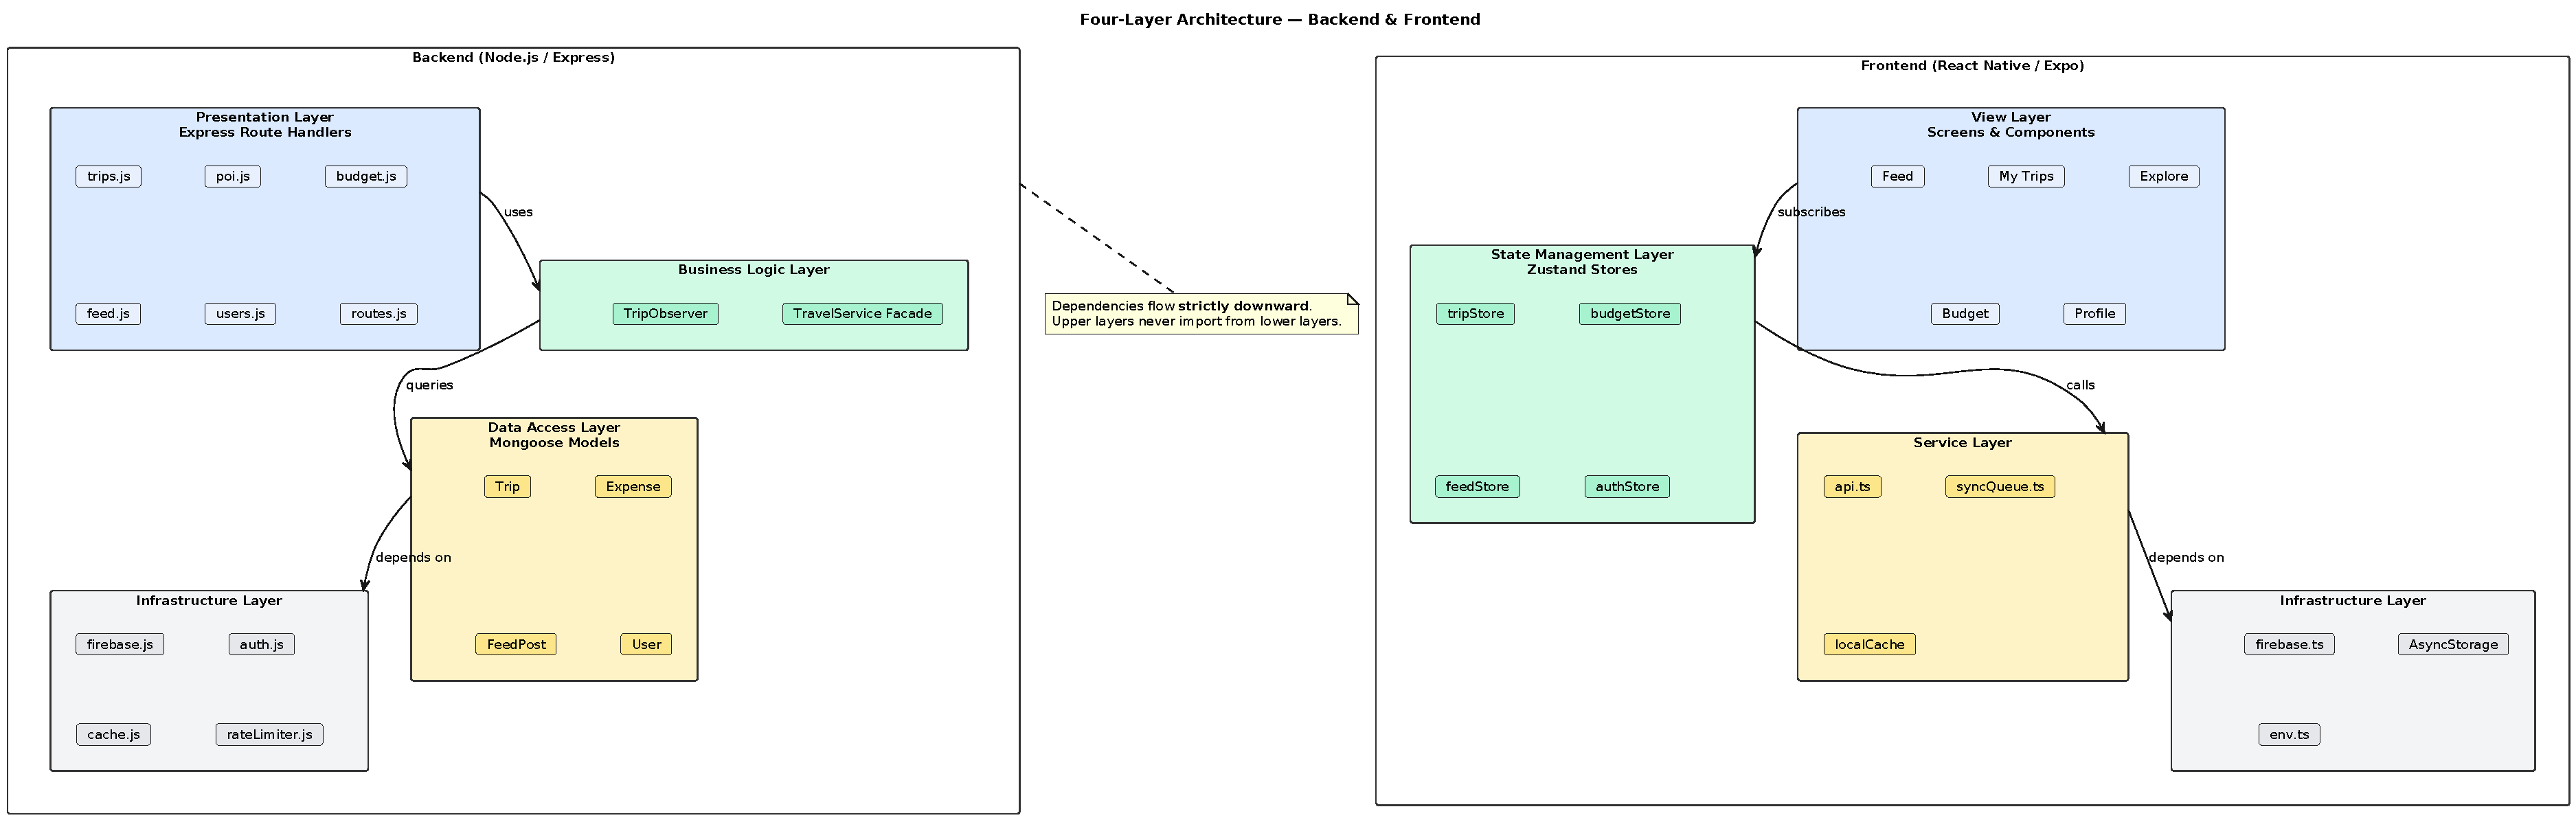
\includegraphics[width=0.90\textwidth]{layered_architecture.pdf}
\caption{Four-layer architecture on both backend and frontend. Dependencies flow strictly downward; upper layers depend on lower layers but never vice versa.}
\label{fig:layered-arch}
\end{figure}

\subsubsection{Reasoning}

The strict layered dependency direction enforces a critical maintainability invariant: changes in infrastructure (e.g., replacing AsyncStorage with MMKV, migrating from node-cache to Redis) propagate upward through at most one layer boundary. Similarly, UI redesigns affect only the view layer. This was validated when the Overpass adapter was disabled: the entire change was confined to the TravelService constructor (business logic layer) --- no route handler, store, or UI component required modification, satisfying NFR-15.

% -----------------------------------------------------------
\subsection{Architectural Tactics --- Summary}
% -----------------------------------------------------------

\begin{longtable}{C{0.5cm} L{3.2cm} L{2.4cm} L{3.0cm} L{3.8cm}}
\toprule
\rowcolor{tableheaderbg}
\thcell{\#} & \thcell{Tactic} & \thcell{Quality Attr.} & \thcell{NFRs Addressed} & \thcell{Key Implementation} \\
\midrule
\endhead
\bottomrule
\endfoot

1 & Multi-layer Response Caching & Performance, Scalability & NFR-01, NFR-06, NFR-07 & \code{localCache}, \code{node-cache}, \code{cacheMiddleware} \\

\rowcolor{tablealtbg}
2 & Authentication \& Secret Proxying & Security & NFR-10, NFR-11, NFR-12 & Firebase JWT, \code{authenticate} middleware, \code{.env} vault \\

3 & Rate Limiting \& Throttling & Scalability & NFR-04, NFR-06 & \code{generalLimiter}, \code{externalApiLimiter} \\

\rowcolor{tablealtbg}
4 & Graceful Degradation \& Fallback & Availability, Reliability & NFR-07, NFR-08, NFR-09 & Provider fallback chain, \code{syncQueue}, offline cache \\

5 & Separation of Concerns (Layered Architecture) & Modifiability & NFR-14, NFR-15 & 4-layer backend/frontend, strict dependency direction \\

\end{longtable}

% ============================================================
\section{Implementation Patterns}
% ============================================================

This section describes two design patterns central to WanderMate's architecture, including their roles, class relationships, and implementation details. Each pattern is illustrated with a UML class diagram.

% -----------------------------------------------------------
\subsection{Pattern 1: Facade + Strategy (TravelService)}
% -----------------------------------------------------------

\subsubsection{Pattern Description}

The \textbf{Facade} pattern provides a unified, simplified interface to a complex subsystem, hiding internal complexity from clients. The \textbf{Strategy} pattern defines a family of algorithms (or service providers), encapsulates each one, and makes them interchangeable. WanderMate combines both patterns in the \code{TravelService} class, which serves as the single point of entry for all POI discovery and route optimisation operations.

\subsubsection{Problem Context}

WanderMate integrates three distinct external APIs for POI data (Google Places, ORS POIs, Overpass/OSM) and one for routing (ORS Directions). Each API has:
\begin{itemize}
  \item A different HTTP protocol (REST, Overpass QL)
  \item A different response schema (JSON with varying field names and nesting)
  \item Different quota limits and pricing models
  \item Different failure modes (rate limiting, geographic restrictions, timeouts)
\end{itemize}

Without a unifying layer, each API consumer (Express route handler) would need to know which provider to call, how to normalise its response, when to fall back, and how to manage caching --- dramatically increasing coupling and making provider changes ripple through the entire codebase.

\subsubsection{Solution Applied}

The \code{TravelService} Facade exposes four high-level methods (\code{searchPOI}, \code{searchByCategory}, \code{getPlaceDetails}, \code{getRoute}) that abstract away all provider-specific logic. Internally, it delegates to interchangeable adapter classes (\code{PlacesAdapter}, \code{ORSAdapter}, and the disabled \code{OverpassAdapter}), each of which implements the same normalised interface but targets a different external API. The Facade also encapsulates caching, fallback orchestration, and error handling.

\subsubsection{UML Class Diagram}

\begin{figure}[H]
\centering
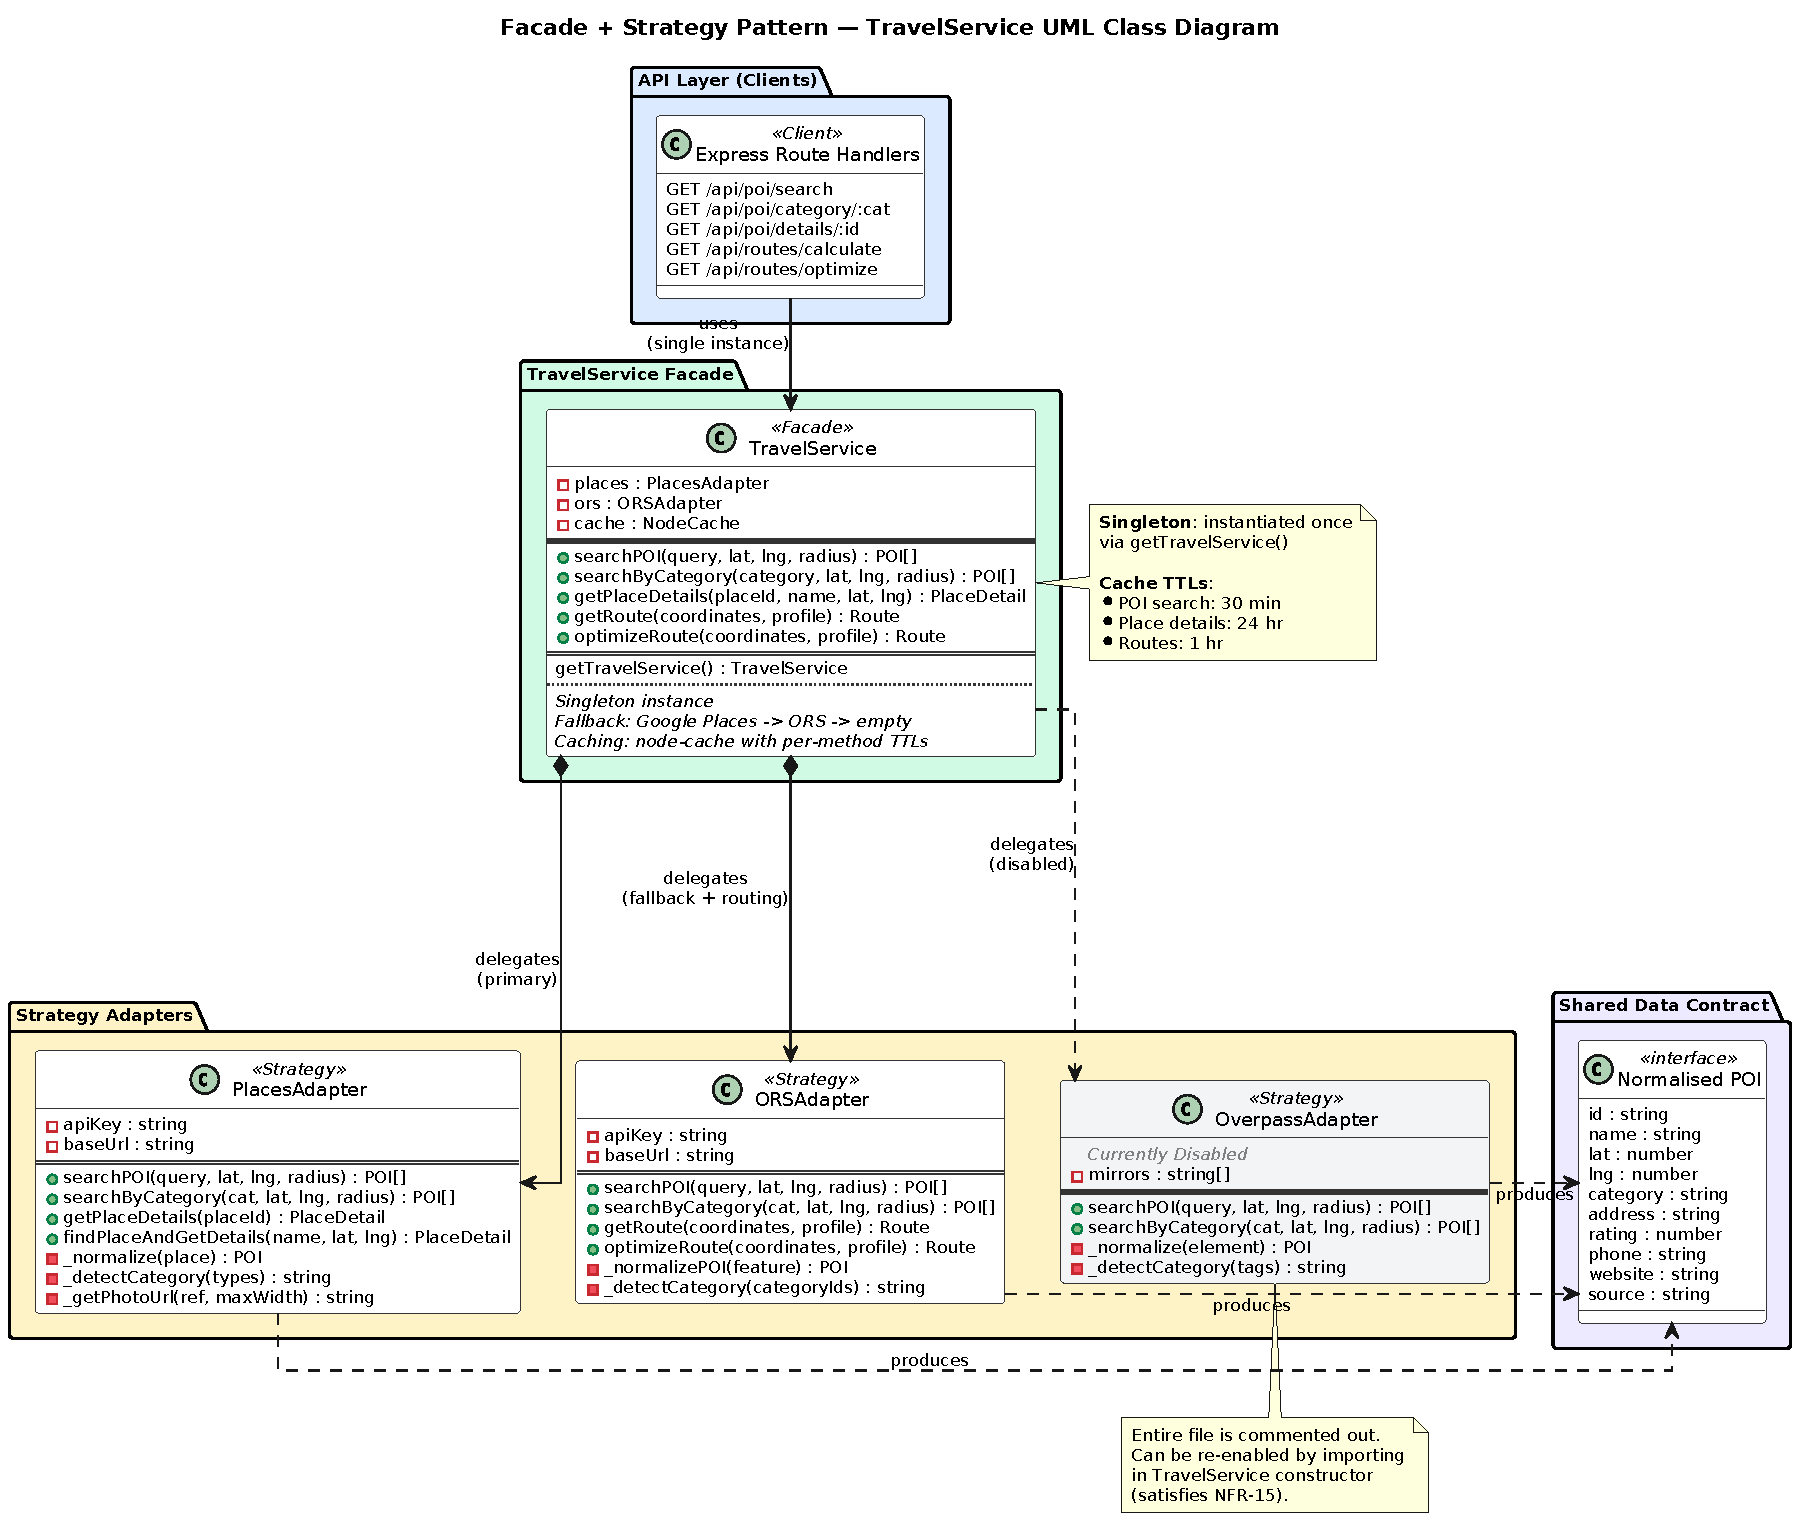
\includegraphics[width=\textwidth]{facade_strategy.pdf}
\caption{UML class diagram: Facade + Strategy pattern in TravelService. Route handlers interact only with the Facade; adapters are interchangeable and produce normalised POI objects.}
\label{fig:facade-strategy}
\end{figure}

\subsubsection{Role Within the Architecture}

\begin{longtable}{L{3.5cm} L{10cm}}
\toprule
\rowcolor{tableheaderbg}
\thcell{Concern} & \thcell{How the Pattern Addresses It} \\
\midrule
\endhead
\bottomrule
\endfoot

Provider Independence & Route handlers call \code{travelService.searchPOI()} without knowing whether the response came from Google Places, ORS, or Overpass. Adding a new provider requires implementing a new adapter class and registering it in the Facade constructor. \\

\rowcolor{tablealtbg}
Fallback Orchestration & The Facade's \code{searchPOI()} method implements the fallback chain (Google $\to$ ORS $\to$ empty). Adapters are unaware of each other; fallback logic is centralised in the Facade. \\

Cache Management & Caching is handled once in the Facade (using \code{node-cache} with per-operation TTLs), preventing duplicate caching logic across adapters and route handlers. \\

\rowcolor{tablealtbg}
NFR-15 Compliance & When the Overpass adapter was disabled, zero changes were needed in route handlers or UI components --- validating the pattern's information-hiding guarantee. \\

\end{longtable}

% -----------------------------------------------------------
\subsection{Pattern 2: Observer Pattern (Real-time Collaboration)}
% -----------------------------------------------------------

\subsubsection{Pattern Description}

The \textbf{Observer} pattern defines a one-to-many dependency between objects, so that when one object (the ``subject'') changes state, all dependent objects (``observers'') are automatically notified and updated. WanderMate uses this pattern extensively for real-time collaborative features, leveraging Firebase Realtime Database as the event bus that connects publishers (backend mutation handlers) and subscribers (frontend Zustand stores).

\subsubsection{Problem Context}

WanderMate supports real-time collaborative trip editing: multiple users can simultaneously modify the same itinerary, and all participants must see changes propagated within 500\,ms (NFR-03). This requires:
\begin{itemize}
  \item A push-based notification mechanism (polling would violate NFR-03's latency target)
  \item Decoupled publishers and subscribers (the backend should not track connected clients)
  \item Multiple independent channels (trip updates, budget updates, auth state changes)
  \item Automatic cleanup on disconnect
\end{itemize}

\subsubsection{Solution Applied}

Firebase Realtime Database acts as the \emph{subject} in the Observer pattern. On the backend, every trip or budget mutation writes an event to a Firebase path (e.g., \code{trips/\{tripId\}}). On the frontend, Zustand stores register \code{onValue} listeners on these paths --- these are the \emph{observers}. When Firebase detects a change, it pushes the update to all connected clients, which then refresh their local state.

\subsubsection{UML Class Diagram}

\begin{figure}[H]
\centering
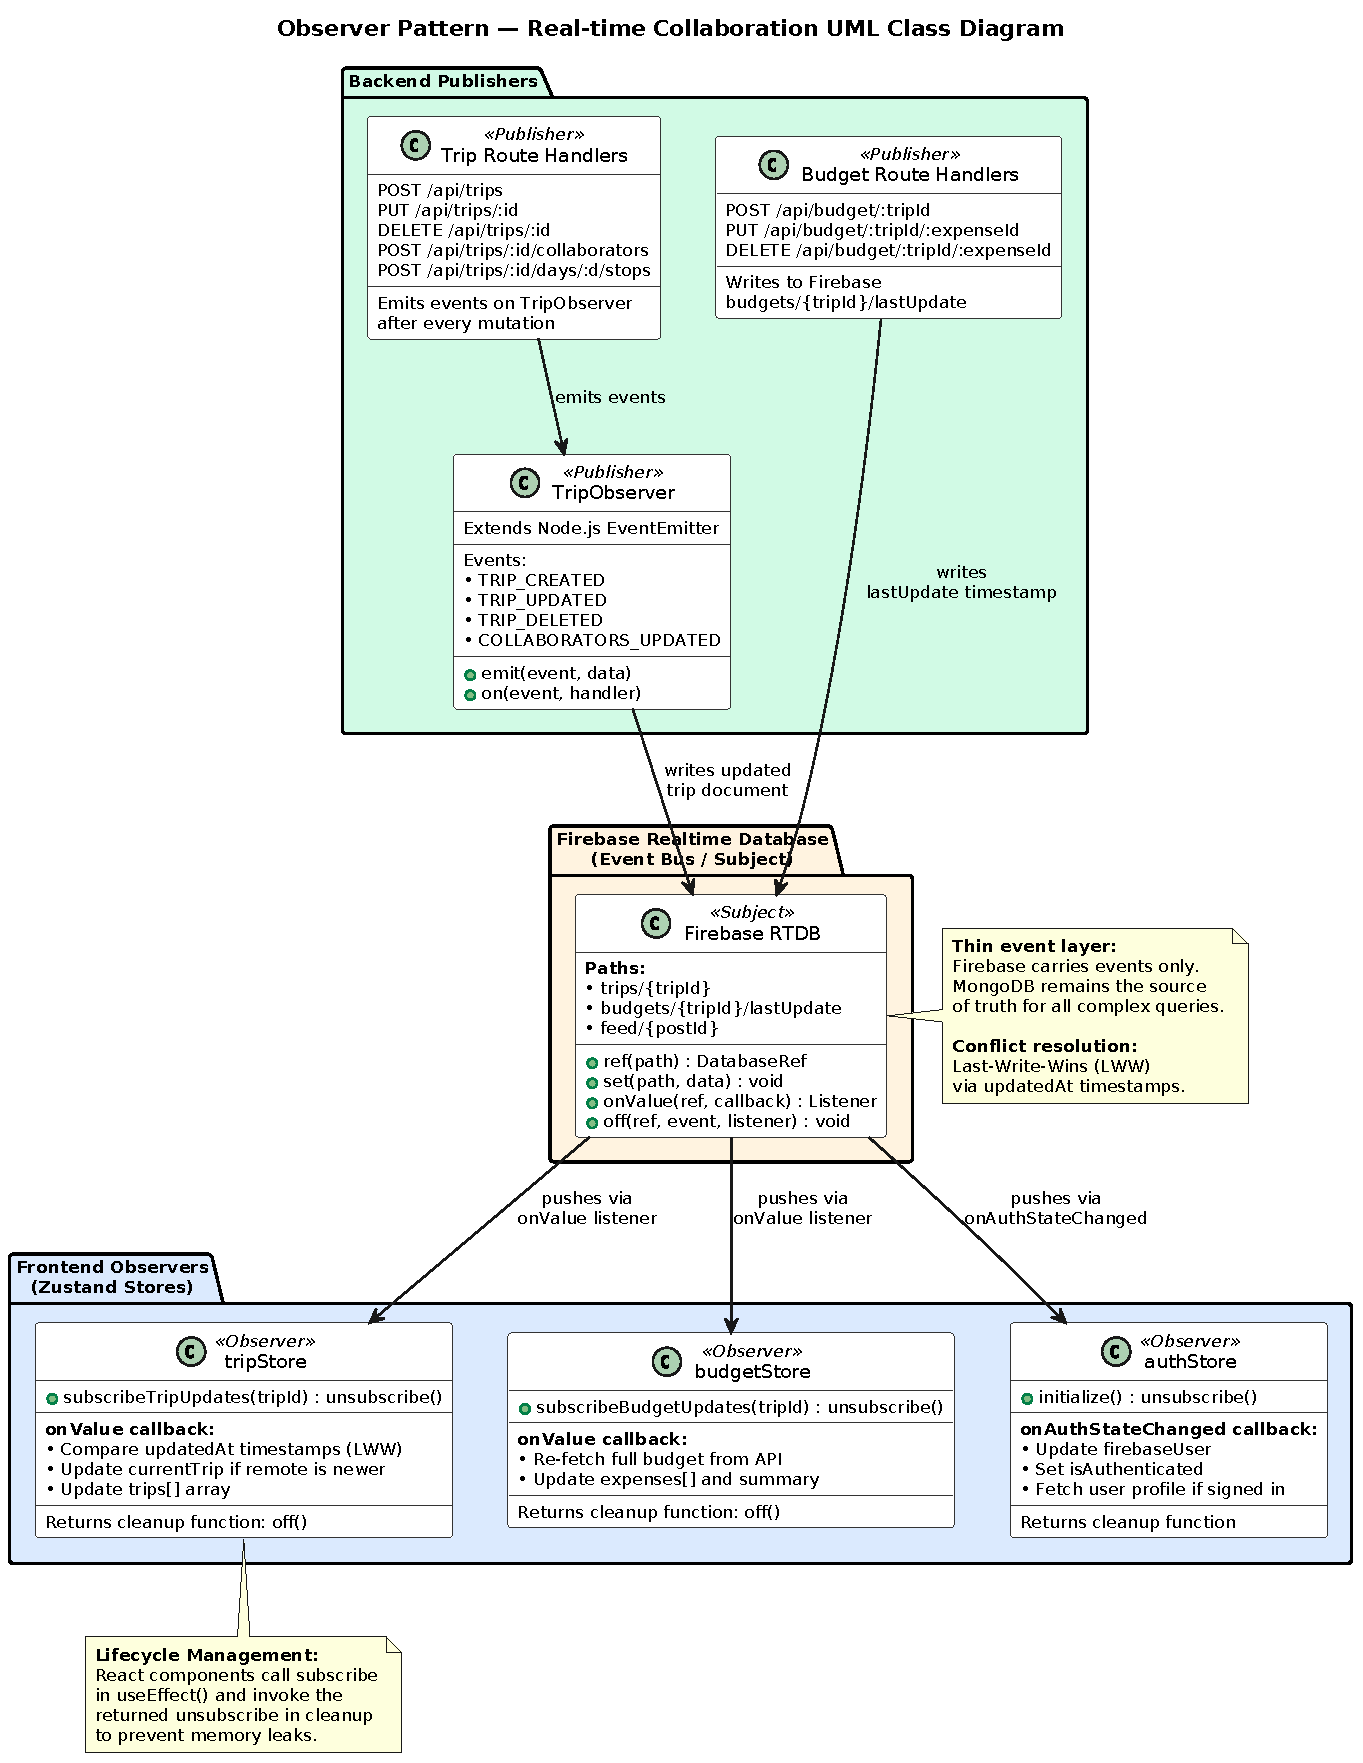
\includegraphics[width=\textwidth]{observer_pattern.pdf}
\caption{UML class diagram: Observer pattern for real-time collaboration. Backend publishers write events to Firebase paths; frontend stores subscribe via \code{onValue} listeners and receive push notifications. Each subscription returns a cleanup function (\code{off()}) to prevent memory leaks.}
\label{fig:observer}
\end{figure}

\subsubsection{Sequence of a Collaborative Edit}

The following sequence describes how a collaborative trip edit propagates to all connected clients:

\begin{enumerate}
  \item \textbf{User A} edits a trip stop via the mobile client. The edit request is sent to the API Gateway.
  \item The \textbf{API Gateway} processes the request: updates the Trip document in MongoDB and emits a \code{TRIP\_UPDATED} event on the \code{TripObserver} EventEmitter.
  \item The \code{TripObserver} event handler catches the event and writes the full updated trip document to \code{trips/\{tripId\}} in \textbf{Firebase Realtime Database}.
  \item Firebase pushes the update to all connected clients that have registered \code{onValue} listeners on that path.
  \item \textbf{User B's} \code{tripStore.subscribeTripUpdates()} callback fires with the new data. The store compares timestamps (Last-Write-Wins) and updates local state if the remote version is newer.
  \item The React Native UI re-renders automatically via Zustand's reactive subscription model.
\end{enumerate}

\subsubsection{Role Within the Architecture}

\begin{longtable}{L{3.5cm} L{10cm}}
\toprule
\rowcolor{tableheaderbg}
\thcell{Concern} & \thcell{How the Pattern Addresses It} \\
\midrule
\endhead
\bottomrule
\endfoot

Real-time Sync (NFR-03) & Firebase's push-based event model ensures updates propagate within 500\,ms, eliminating the latency overhead of polling. \\

\rowcolor{tablealtbg}
Decoupled Communication & Publishers (backend route handlers) and subscribers (frontend stores) have no direct dependency on each other. The backend writes to Firebase paths without knowing which or how many clients are listening. \\

Multi-channel Events & Three independent observation channels (trip updates, budget updates, auth state) operate concurrently without interference, each managed by its own Firebase path and Zustand store. \\

\rowcolor{tablealtbg}
Resource Cleanup & Every \code{subscribe*} method returns an \code{unsubscribe} function (wrapping Firebase's \code{off()} method). React components call this in their cleanup effect (\code{useEffect} return), preventing memory leaks and orphan listeners. \\

Conflict Resolution & The \code{tripStore} observer implements last-write-wins (LWW) by comparing \code{updatedAt} timestamps before applying incoming state: \code{if (remote.updatedAt >= local.updatedAt)} --- providing eventual consistency without complex merge logic. \\

\end{longtable}

% ============================================================
\section{Relationship Between Tactics and Patterns}
% ============================================================

The architectural tactics and design patterns are not independent --- they reinforce each other in a cohesive architectural strategy. The following diagram and table illustrate the relationships:

\begin{figure}[H]
\centering
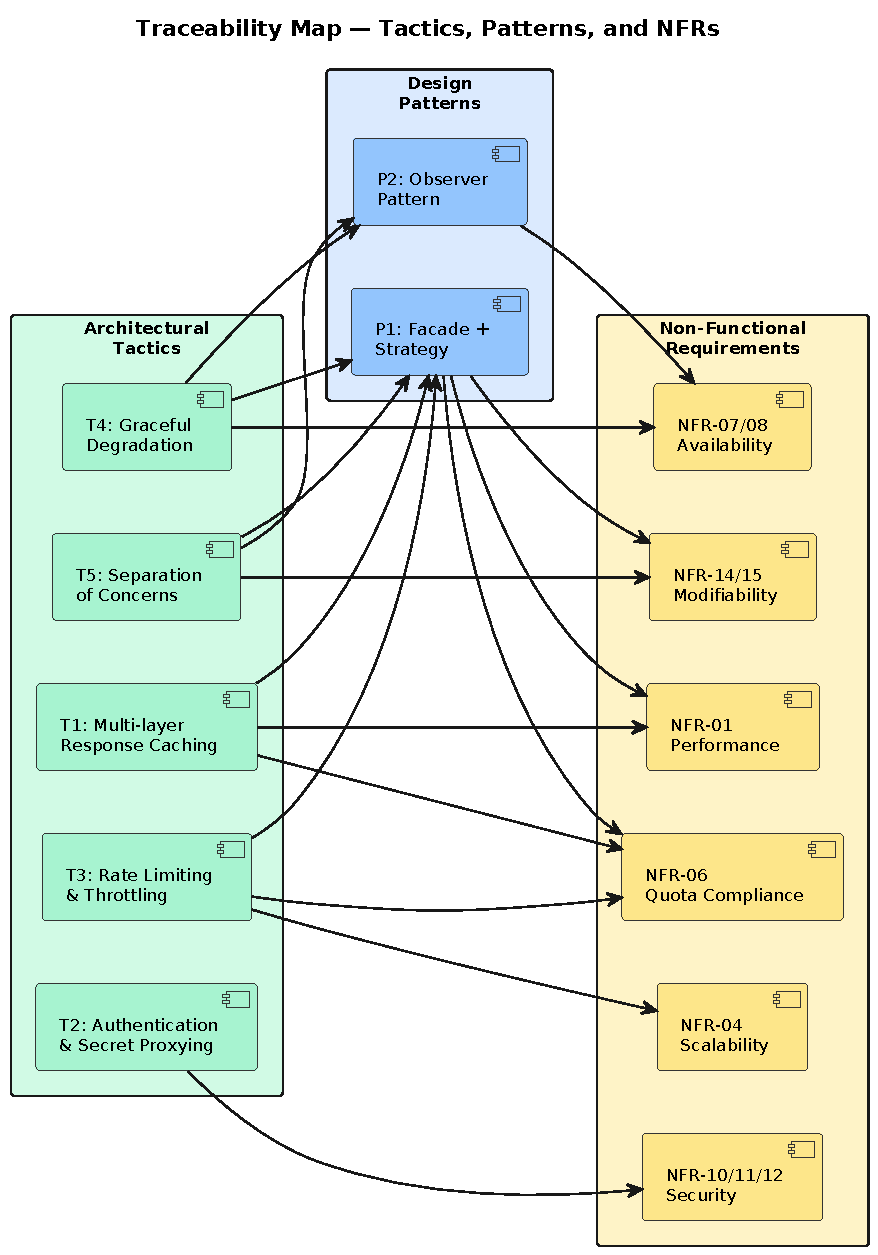
\includegraphics[width=\textwidth]{traceability_map.pdf}
\caption{Traceability map: architectural tactics (green) and design patterns (blue) are linked to the non-functional requirements (amber) they jointly satisfy. Dashed lines show mutual reinforcement between tactics and patterns.}
\label{fig:traceability}
\end{figure}

\begin{longtable}{L{3.5cm} L{3.5cm} L{6.5cm}}
\toprule
\rowcolor{tableheaderbg}
\thcell{Tactic} & \thcell{Enabled By Pattern} & \thcell{Relationship} \\
\midrule
\endhead
\bottomrule
\endfoot

T1: Multi-layer Caching & Facade + Strategy & Caching is centralised in the Facade, applied once regardless of which adapter produced the result. \\

\rowcolor{tablealtbg}
T3: Rate Limiting & Facade + Strategy & Rate limiting is applied at the gateway layer, before the Facade is invoked. The Facade's unified interface means a single rate limiter covers all provider calls. \\

T4: Graceful Degradation & Facade + Strategy & The fallback chain (Google $\to$ ORS $\to$ empty) is orchestrated inside the Facade. Adapters are unaware of fallback logic. \\

\rowcolor{tablealtbg}
T4: Graceful Degradation & Observer Pattern & The Observer pattern enables real-time state refresh after reconnection, complementing the sync queue's offline mutation queuing. \\

T5: Layered Architecture & Both Patterns & Both patterns enforce strict layer boundaries: the Facade isolates adapters from route handlers; the Observer decouples publishers from subscribers via Firebase. \\

\end{longtable}

% ============================================================
\section{Conclusion}
% ============================================================

WanderMate's architecture is shaped by a deliberate set of five architectural tactics and two design patterns that collectively address the system's most demanding non-functional requirements:

\begin{enumerate}
  \item \textbf{Multi-layer Response Caching} ensures sub-2-second response times and free-tier quota compliance through a three-tier cache hierarchy (client $\to$ service $\to$ middleware).

  \item \textbf{Authentication \& Secret Proxying} protects API keys from mobile bundle extraction and enforces Firebase JWT verification on every request via the API Gateway.

  \item \textbf{Rate Limiting \& Throttling} prevents resource exhaustion and quota overruns through dual-tier per-IP rate limits.

  \item \textbf{Graceful Degradation \& Fallback} ensures continuous availability through provider fallback chains and offline-first client caching with a persistent sync queue.

  \item \textbf{Separation of Concerns via Layered Architecture} enforces strict dependency direction across four layers on both backend and frontend, enabling independent evolution and provider swappability.
\end{enumerate}

The \textbf{Facade + Strategy} pattern (TravelService) unifies multiple external API providers behind a single interface, centralising caching, fallback, and quota management. The \textbf{Observer} pattern (Firebase Realtime Database subscriptions) enables real-time collaborative editing with sub-500ms propagation latency, decoupled publisher--subscriber communication, and automatic resource cleanup.

These tactics and patterns are not applied in isolation --- they form a mutually reinforcing architectural strategy where the Facade centralises the application of caching, rate limiting, and degradation tactics, and the Observer pattern complements offline-first availability with real-time synchronisation on reconnect.

\end{document}
